\documentclass[tikz,border=10pt]{standalone}
\usepackage{tikz}
\usetikzlibrary{matrix}

\tikzset{
  cell/.style={draw=black!70, line width=1.0pt, minimum width=5.3cm, minimum height=1.1cm, align=center, text width=4.8cm},
  head/.style={cell, draw=blue!70!black, line width=1.2pt},
  left/.style={cell, draw=green!50!black, line width=1.2pt}
}

\begin{document}
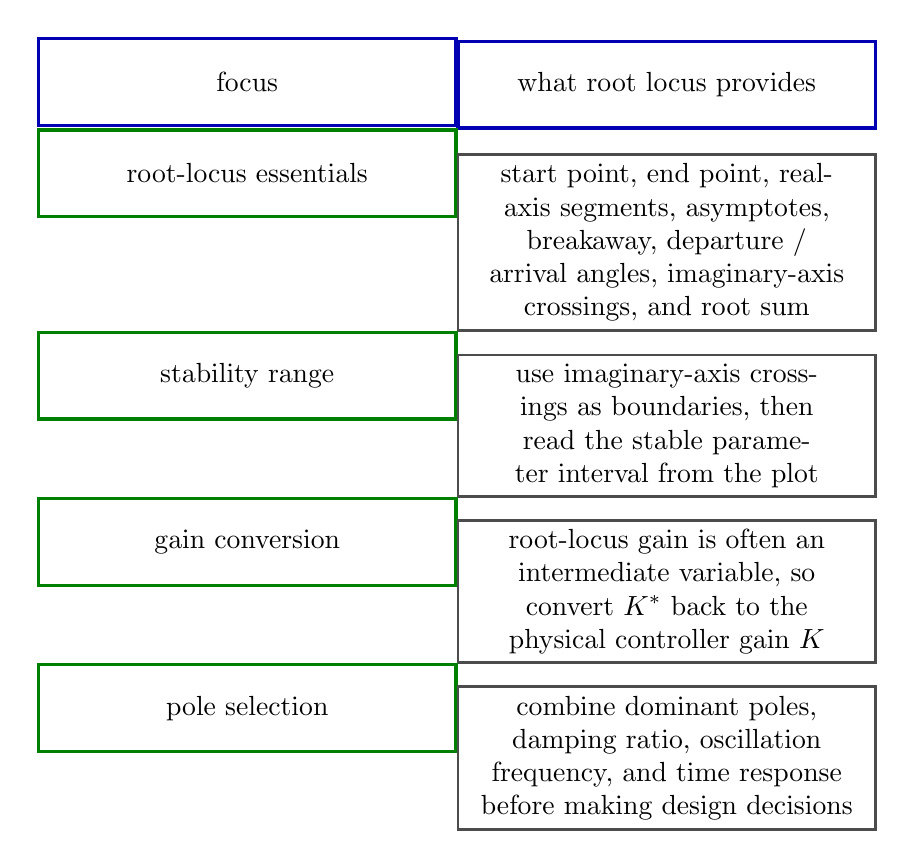
\begin{tikzpicture}
  \matrix[matrix of nodes, nodes in empty cells, row sep=-\pgflinewidth, column sep=-\pgflinewidth] {
    \node[head] {focus}; & \node[head] {what root locus provides}; \\
    \node[left] {root-locus essentials}; & \node[cell] {start point, end point, real-axis segments, asymptotes, breakaway, departure / arrival angles, imaginary-axis crossings, and root sum}; \\
    \node[left] {stability range}; & \node[cell] {use imaginary-axis crossings as boundaries, then read the stable parameter interval from the plot}; \\
    \node[left] {gain conversion}; & \node[cell] {root-locus gain is often an intermediate variable, so convert $K^\ast$ back to the physical controller gain $K$}; \\
    \node[left] {pole selection}; & \node[cell] {combine dominant poles, damping ratio, oscillation frequency, and time response before making design decisions}; \\
  };
\end{tikzpicture}
\end{document}
